\documentclass{beamer}
\usetheme{Warsaw}

\setbeamercolor{normal text}{fg=white,bg=black!90}
\setbeamercolor{structure}{fg=white}

\setbeamercolor{alerted text}{fg=red!85!black}

\setbeamercolor{item projected}{use=item,fg=black,bg=item.fg!35}

\setbeamercolor*{palette primary}{use=structure,fg=structure.fg}
\setbeamercolor*{palette secondary}{use=structure,fg=structure.fg!95!black}
\setbeamercolor*{palette tertiary}{use=structure,fg=structure.fg!90!black}
\setbeamercolor*{palette quaternary}{use=structure,fg=structure.fg!95!black,bg=black!80}

\setbeamercolor*{framesubtitle}{fg=white}

\setbeamercolor*{block title}{parent=structure,bg=black!60}
\setbeamercolor*{block body}{fg=black,bg=black!10}
\setbeamercolor*{block title alerted}{parent=alerted text,bg=black!15}
\setbeamercolor*{block title example}{parent=example text,bg=black!15}

\DeclareMathOperator*{\mymax}{max}
\DeclareMathOperator*{\argmax}{arg\,max}
\DeclareMathOperator*{\argmin}{arg\,min}
\DeclareMathOperator*{\ForAll}{\bigwedge}
\DeclareMathOperator*{\Exists}{\bigvee}
\newcommand{\W}{\mathcal{W}}

\newcommand*\kreis[2]{\unitlength0.7ex\begin{picture}(2.5,2.5)%


\color{#2}%
\put(0.75,0.75){\circle*{3}}%
\color{black}%
\put(0.75,0.75){\circle{3}}%
\put(0.7,0.7){\makebox(0,0){#1}}\end{picture}}
\newcommand\itplus{\kreis{$+$}{green}}
\newcommand\itminus{\kreis{$-$}{red}}
\newcommand\prob[2]{\ensuremath{p_{\mathrm{#1}}\left( #2 \right)}}
\newcommand\bedprob[3]{\ensuremath{p_{\mathrm{#1}}\left( #2 \left|#3\right. \right)}}

\newcommand\etal{et.\,al.}

\usepackage[english]{babel}
% avant, courier, chancery, times, palatino, bookman, 
% newcent, utopia, charter
%\usepackage{times}

\usepackage{natbib}
\usepackage{booktabs}
\usepackage{tabularx}

\usepackage[latin1]{inputenc}
\usepackage[T1]{fontenc}
\usepackage{multicol}
\usepackage{mdwtab}
\usepackage{booktabs}
\usepackage{tabularx}
\usepackage{txfonts,textcomp}
\usepackage{amsmath}
\usepackage{amsfonts}

\setlength\parindent{0cm}
\setlength\parskip{2mm}
\setbeamerfont{gross}{size=\large}
\setbeamerfont{quetsch}{size=\tiny}
\setbeamerfont{klein}{size=\footnotesize}
\newcommand\w[1]{\mathbf{#1}}

% example list spacing
\newcommand\ml{\setlength\itemindent{-11mm}}

	\title{Structured Prediction and PyStruct} 
    \author[short]{Andreas M\"uller}%

	\begin{document}

	\begin{frame}[plain]
		\titlepage
	\end{frame}

    \section{Motivation}
    % output space combinatorial
    % output space depends on input space
    % model correlations
    \begin{frame}
        \frametitle{Multi-Label Classification}
    \end{frame}

    \begin{frame}
        \frametitle{Sequence Tagging}
        % voice recognition
        % part of speech tagging
        % action recognition
    \end{frame}

    \begin{frame}
        \frametitle{Predicting Parse Trees}
    \end{frame}

    \begin{frame}
        \frametitle{Semantic Images Segmentation}
    \end{frame}

    \begin{frame}
        \frametitle{Predicting Structured Objects}
        \[f(x, w) := \argmax_{y \in \mathcal{Y}}  g(x, y, w) \]
        \begin{visibleenv}<2->
        If you like:
        \[\argmax_{y \in \mathcal{Y}}  p(y|x, w) \]
        \end{visibleenv}
        
        \begin{visibleenv}<3>
        \[f(x, w) := \argmax_{y \in \mathcal{Y}}  w^T \psi(x, y) \]
        \end{visibleenv}
    \end{frame}

    \section{Inference and Factor Graphs}
    \begin{frame}
        \frametitle{Predicting discrete vectors}
    \end{frame}

    \begin{frame}
        \frametitle{Factor Graphs}
        % general functions
        % then linear svm
    \end{frame}

    \begin{frame}
        \frametitle{Inference in Trees}
    \end{frame}

    \begin{frame}
        \frametitle{Inference in Gerneral Graphs}
    \end{frame}

    \section{Learning}
    \begin{frame}
        \frametitle{Probabilistic Learning}
    \end{frame}
    \begin{frame}
        \frametitle{Max-Margin Learning}
    \end{frame}


    \section{PyStruct}
    \begin{frame}
        \frametitle{Simple structured prediction}
        % Learner
        % Model
        % Inference
    \end{frame}

    \begin{frame}
        \frametitle{Example OCR}
    \end{frame}

    \begin{frame}
        \frametitle{Example Snake}
    \end{frame}

    \begin{frame}
        \begin{center}
            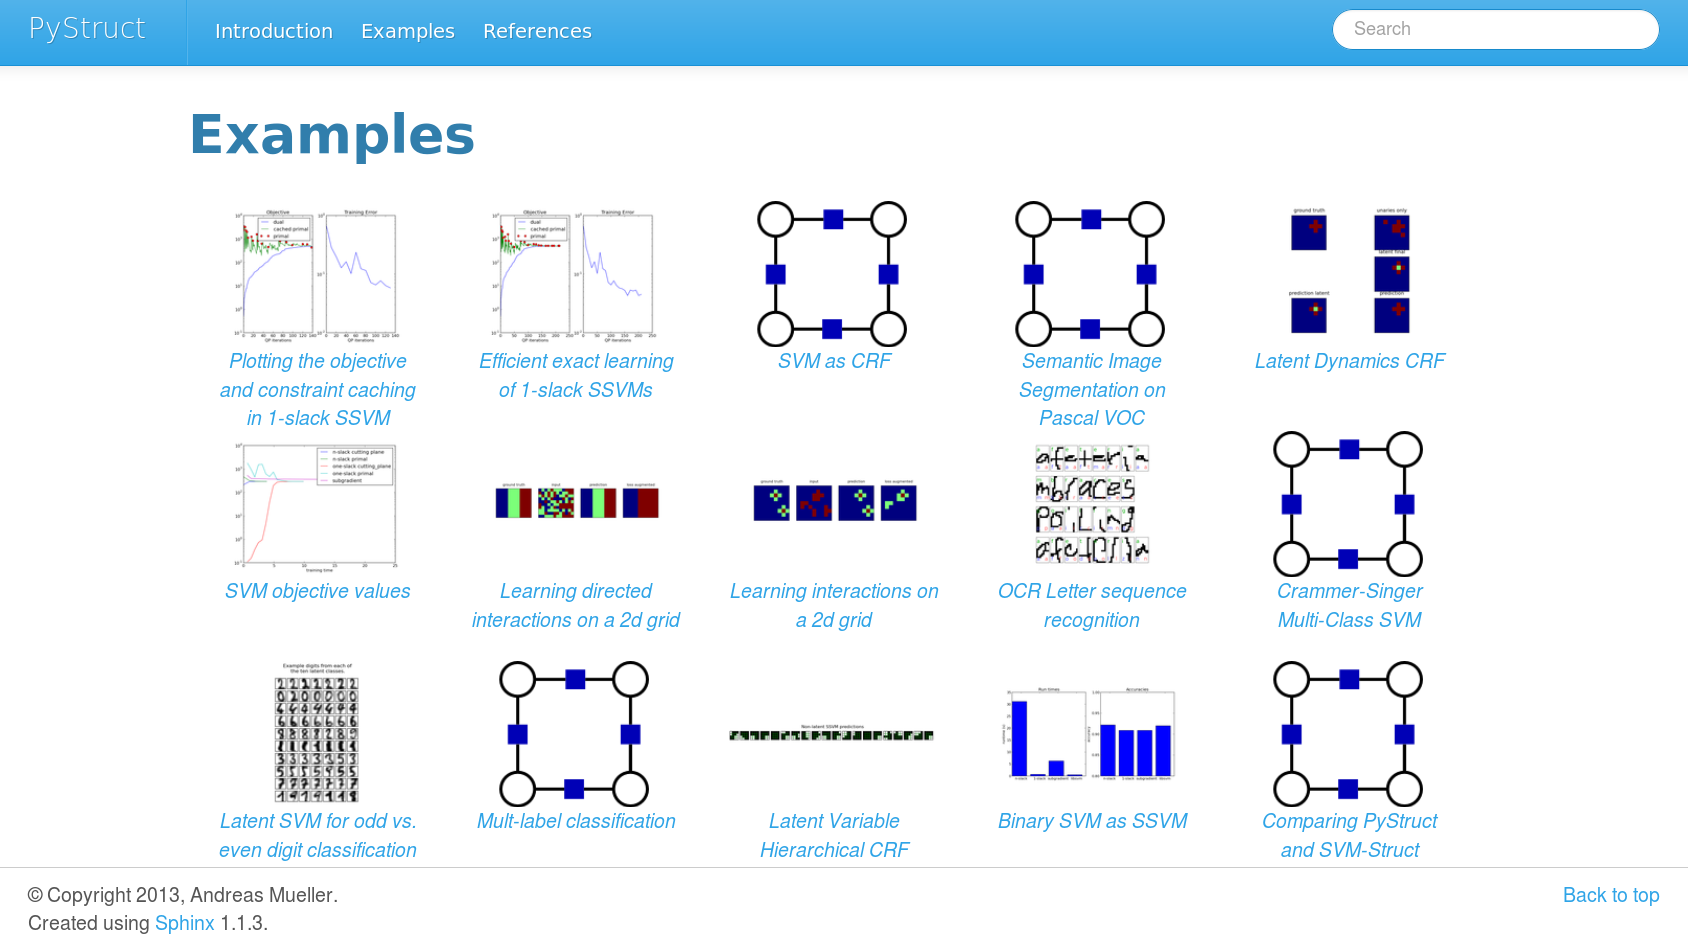
\includegraphics[width=\linewidth]{images/example_gallery}\\
            http://pystruct.github.io
        \end{center}
    \end{frame}
    
	\end{document}
